\documentclass[../documentation.tex]{subfiles}

\begin{document}

\subsection{Wallet}

Each user owns a pair of private and public key.
Transactions must be signed by the private key. Users
can send their money to another address, which is given by the public key.

\subsection{Block}

All the transactions broadcasted to the network are grouped into blocks, which contain

\begin{itemize}
    \item Transactions hash
    \item Timestamp
    \item difficulty (PoW)
    \item Nonce (PoW)
    \item Previous block hash
    \item Number of transactions
\end{itemize}

With each block being confirmed, the blockchain is created
and transactions are confirmed.

\subsection{Proof of Work}

Proof-of-Work (PoW) is a cryptographic proof that a party has spent
a certian amount of computational effort.

When a miner solves the puzzle, the current block is archived, a new
block is generated and all the transactions in the previous block are confirmed.
The miner is then rewarded by the system.

\subsection{Proof of Stake}

Proof-of-Stake (PoS) is a consensus mechanism that help choose witch participants
are rewarded.

When blockchain participants verify that a transaction is legitimate and add it
to the blockchain, participants have archived consensus.

\subsection{Smart Contracts}

Smart contracs are programs associated with an address and run on the blockchain.
The nodes run code from the contract program at a relevant event, such as a received transation.

Users can interact with the contract via transactions. Contracts can often interact with other contracts
and some of them are Turing-complete.

%\subsubsection{Deployment}
%
%A smart contract is deployed by sending a transaction to the blockchain which includes the compiled program
%as well as a special receiver address.
%
%The program is added to the current block. When the block is added to the blockchain, the contract
%will execute one time to set its initial state, at which point the smart contract will now be valid and running.

\subsection{Difficulty (PoW)}

If we want the time gap between two mined blocks to be approximately
\(N\) units of time, we need adjust the difficulty of the mining process every 
\(M\) units of time such that

\[
    \text{difficulty}_\text{current} =
    \text{difficulty}_\text{previous}
    \cdot \frac{M}{\Delta (\frac{M}{N})}
\]

where \(\Delta (x)\) is the units of time to mine the last \(x\) blocks.

Or we could adjust the difficulty \(N\) blocks

\[
    \text{difficulty}_\text{current} =
    \text{difficulty}_\text{previous}
    \cdot \frac{N \cdot k}{\Delta(k)}
\]

where \(k\) is the number of last blocks on which you want to
base the adjustment on. These two formulas are the same.

\subsection{Mempool}

The mempool is the place where uncofirmed transactions
wait to be confirmed.
When a transaction is broadcasted and received by the nodes,
if valid, it is put in the mempool.
When a new block is created, up to X transactions are removed from the
mempool and will be included in the next block.

\subsection{Deployment}

To deploy a transaction a node has to broadcast it to his peers.
To avoid flooding of the network, a node will only broadcast
the same transaction once (as long as the transaction is still in the mempool).

\subsection{Merkle Trees}

The hash of all the transaction within a block if often
computed using a merkle tree.

A Markle tree or hash tree is a tree where each node contains the hash of its children, and every leaf contains
the hash of a data block

The root of the tree is the transactions hash.

\begin{center}
    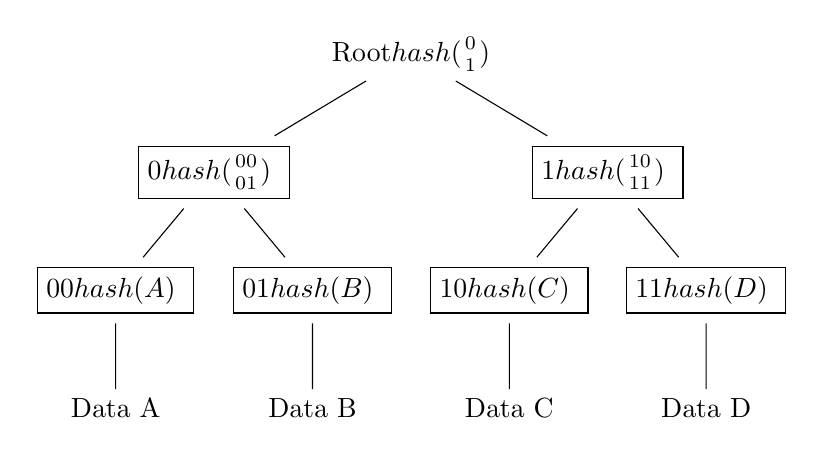
\begin{tikzpicture}[
        level 1/.style = {sibling distance = 5cm},
        level 2/.style = {sibling distance = 2.5cm}
    ]
    \node {\doublebox{\makecell{Root \\ \(\text{hash}({0\atop 1})\) }}}
        child {
            node {\fbox{\makecell{0 \\ \(\text{hash}({00\atop 01})\) }}}
            child {
                node {\fbox{\makecell{00 \\ \(\text{hash}(A)\) }}}
                child {
                    node {\ovalbox{Data A}}
                }
            }
            child {
                node {\fbox{\makecell{01 \\ \(\text{hash}(B)\) }}}
                child {
                    node {\ovalbox{Data B}}
                }
            }
        }
        child {
            node {\fbox{\makecell{1 \\ \(\text{hash}({10\atop 11})\) }}}
            child {
                node {\fbox{\makecell{10 \\ \(\text{hash}(C)\) }}}
                child {
                    node {\ovalbox{Data C}}
                }
            }
            child {
                node {\fbox{\makecell{11 \\ \(\text{hash}(D)\) }}}
                child {
                    node {\ovalbox{Data D}}
                }
            }
        };
    \end{tikzpicture}
\end{center}

\end{document}